\documentclass[11pt,a4paper,oneside]{report}
\newcommand{\ReportShortTitle}{When Is a Backtest Real?}
% Shared layout: title page, executive summary, centred red chapter titles,
% blue small-caps sections, running header. Compile with pdflatex.
\usepackage[T1]{fontenc}
\usepackage[utf8]{inputenc}
\usepackage{charter}
\usepackage[scaled=0.92]{helvet}
\usepackage{amsmath,amssymb}
\usepackage[a4paper,margin=2.3cm,headheight=28pt]{geometry}
\usepackage{graphicx,booktabs,xcolor,titlesec,fancyhdr,enumitem,listings,float,caption}
\usepackage[hidelinks]{hyperref}
\definecolor{navy}{HTML}{0B3A5B}
\definecolor{accent}{HTML}{D6312B}
\definecolor{secblue}{HTML}{1E6A8D}
\definecolor{codebg}{HTML}{F3F1EA}
\setlength{\parindent}{1.5em}
\setlength{\parskip}{3pt}
\linespread{1.05}
\newcommand{\ornament}{\par\vspace{2pt}{\centering\color{accent}\rule{2.2cm}{0.4pt}\hspace{2pt}\rule[-1pt]{1.2cm}{2.2pt}\hspace{2pt}\rule{2.2cm}{0.4pt}\par}\vspace{6pt}}
\titleformat{\chapter}[display]{\centering\sffamily\bfseries\color{accent}}{\Large\thechapter}{2pt}{\LARGE\MakeUppercase}[\ornament]
\titlespacing*{\chapter}{0pt}{-10pt}{14pt}
\titleformat{name=\chapter,numberless}[display]{\centering\sffamily\bfseries\color{accent}}{}{0pt}{\LARGE\MakeUppercase}[\ornament]
\titlespacing*{name=\chapter,numberless}{0pt}{-10pt}{14pt}
\titleformat{\section}{\Large\scshape\color{secblue}}{\thesection}{0.6em}{}[{\color{secblue}\vspace{-4pt}\rule{1.1cm}{2pt}}]
\titleformat{\subsection}{\large\scshape\color{secblue}}{\thesubsection\enspace$\bullet$}{0.5em}{}
\pagestyle{fancy}
\fancyhf{}
\fancyhead[L]{\color{navy}\scshape\small\ReportShortTitle}
\fancyfoot[C]{\color{navy}\rule[3pt]{0.5cm}{0.4pt}\\\thepage}
\renewcommand{\headrulewidth}{0pt}
\fancypagestyle{plain}{\fancyhf{}\fancyhead[L]{\color{navy}\scshape\small\ReportShortTitle}\fancyfoot[C]{\color{navy}\rule[3pt]{0.5cm}{0.4pt}\\\thepage}\renewcommand{\headrulewidth}{0pt}}
\captionsetup{font=small,labelfont=sc}
\lstset{basicstyle=\ttfamily\footnotesize,backgroundcolor=\color{codebg},frame=none,
  keywordstyle=\color{accent},commentstyle=\color{gray},numbers=left,
  numberstyle=\tiny\color{gray},language=Python,breaklines=true,columns=fullflexible,xleftmargin=1.5em}
\newcommand{\maketitlepage}[5]{% title, subtitle, date, author, repo
\begin{titlepage}\centering
\vspace*{5cm}
{\sffamily\bfseries\color{navy}\fontsize{26}{32}\selectfont\MakeUppercase{#1}\par}
\vspace{2.2cm}
{\sffamily\bfseries\color{navy}\Large #2\par}
\vspace{4.5cm}
{\color{navy}\large #3\par}
\vspace{4pt}{\color{navy}\rule{1.2cm}{2pt}\par}\vspace{8pt}
{\color{navy}\large #4\par}
\vspace{6pt}{\color{navy}\small\texttt{#5}\par}
\vfill
{\color{navy}\small Independent research project\par}
\end{titlepage}}


\begin{document}
\maketitlepage{When Is a Backtest Real?}
{Selection Bias, Multiple Testing and the Probability of Backtest Overfitting, Measured on Synthetic Strategies}
{October 2026}{Stéphane N'Da}{github.com/StephaneMian/backtest-overfitting}

\chapter*{Executive Summary}
\thispagestyle{plain}

A systematic researcher rarely tests one idea. Parameters are varied, signals are combined, universes are filtered, and the backtest that is finally shown is the best of many. Each test is honest on its own; the selection is what creates the illusion. This project quantifies that illusion with synthetic strategies whose true Sharpe ratio is known, so that every statistical tool can be judged against the ground truth.

The first result sets the scale. With five years of daily data and no signal at all, the best of 100 strategies shows an annualised Sharpe ratio of 1.11 on average, and the best of 1\,000 shows 1.44, with a 95th percentile of 1.71. An extreme-value approximation predicts these averages within 5\%, so the expected level of luck can be computed before looking at any result.

The second result concerns the decision rule. A standard test applied to the selected strategy, the probabilistic Sharpe ratio (PSR) above 95\%, declares the best of 100 noise strategies significant in 99.5\% of simulations. The deflated Sharpe ratio, which replaces the zero benchmark by the expected maximum under the null, does so in 0.5\% of simulations. The price of that protection is power: a single genuine strategy with a Sharpe ratio of 1.0 hidden among 99 noise strategies is detected only 1.5\% of the time, and 55\% of the time at a Sharpe of 2.0. Five years of data cannot separate a good strategy from the luck of 100 trials.

The third result compares corrections across a universe of 1\,000 strategies of which 50 are real. Without correction, 56\% of the strategies declared significant are false. Bonferroni and Holm keep the false discovery proportion at 2.6\% but recover only 5\% of the real strategies; Benjamini--Hochberg keeps it at 5.6\% and recovers 13\%. Finally, the probability of backtest overfitting (PBO) separates a noise universe (average 0.47) from one containing a real strategy (average 0.23), but it varies by 0.15 to 0.19 from one dataset to another, so a single PBO value should be read as a noisy estimate and not as a verdict.

\tableofcontents

%--------------------------------------------------------------------------
\chapter{Why Selection Changes the Statistics}

\section{The quantity being tested}
Let $r_1,\dots,r_T$ be the daily excess returns of a strategy with mean $\mu$ and standard deviation $s$. The per-period Sharpe ratio is estimated by $\widehat{SR}=\bar r/\hat s$ and annualised by the factor $\sqrt{252}$. For i.i.d.\ returns with skewness $\gamma_3$ and kurtosis $\gamma_4$, the estimator is asymptotically normal with variance
\begin{equation}\label{eq:var}
\mathrm{Var}\big(\widehat{SR}\big)\approx\frac{1-\gamma_3\,SR+\frac{\gamma_4-1}{4}SR^2}{T-1},
\end{equation}
which reduces to $(1+SR^2/2)/(T-1)$ for normal returns (Lo 2002, Mertens 2002). For five years of daily data the standard error of the annualised Sharpe ratio of a zero-mean strategy is about $1/\sqrt 5\approx0.45$. A single honest backtest with an annualised Sharpe of 0.9 is therefore only two standard errors away from zero.

\section{Probabilistic and deflated Sharpe ratios}
The probabilistic Sharpe ratio is the probability, under the asymptotic distribution above, that the true Sharpe ratio exceeds a benchmark $SR^*$:
\begin{equation}
\mathrm{PSR}(SR^*) = \Phi\!\left(\frac{\widehat{SR}-SR^*}{\widehat{\mathrm{se}}}\right).
\end{equation}
With $SR^*=0$ this is a one-sided $z$-test. It is correct for a strategy fixed in advance and wrong for the best of $N$ strategies, because the maximum of $N$ noisy estimates is biased upwards.

For $N$ independent null estimates with standard deviation $v$, extreme-value theory gives
\begin{equation}\label{eq:emax}
\mathbb E\big[\max_i \widehat{SR}_i\big]\approx v\left[(1-\gamma)\,\Phi^{-1}\!\Big(1-\frac1N\Big)+\gamma\,\Phi^{-1}\!\Big(1-\frac1{Ne}\Big)\right],
\end{equation}
where $\gamma\approx0.5772$ is the Euler--Mascheroni constant. The deflated Sharpe ratio (Bailey and López de Prado 2014) is the PSR of the selected strategy computed with this expected maximum as benchmark. In the experiments $v$ is estimated as the cross-sectional standard deviation of the $N$ Sharpe ratios.

\section{Families of tests}
When many strategies are tested and all significant ones are kept, the relevant error rates are the family-wise error rate (FWER), the probability of at least one false discovery, and the false discovery rate (FDR), the expected fraction of false discoveries among the rejections. Bonferroni and Holm control the FWER; Benjamini--Hochberg controls the FDR, which is less strict and more useful when some false positives are acceptable as long as they remain a small fraction of the portfolio of signals.

\section{Combinatorially symmetric cross-validation}
The PBO method (Bailey, Borwein, López de Prado and Zhu 2017) does not require a count of trials. The $T\times N$ matrix of returns is cut into $S$ contiguous blocks. For each of the $\binom{S}{S/2}$ ways to choose half of the blocks as in-sample, the best in-sample strategy is selected and its rank $\omega\in(0,1)$ among all strategies out of sample is recorded, together with the logit $\lambda=\ln\big(\omega/(1-\omega)\big)$. PBO is the fraction of splits with $\lambda\le0$, that is, where the selected strategy ends in the bottom half out of sample.

\section{Experimental design}
All strategies are simulated as i.i.d.\ daily returns with 1\% daily volatility and a prescribed true annualised Sharpe ratio, zero unless stated. Because the truth is known, every rejection can be labelled as true or false. The simulations are seeded and the script that produces all figures and tables is included in the repository.

%--------------------------------------------------------------------------
\chapter{Results}

\section{The best of N strategies with no signal}
Figure~\ref{fig:max} shows the annualised Sharpe ratio of the best of $N$ zero-mean strategies over five years, averaged over 200 simulations.

\begin{figure}[H]\centering
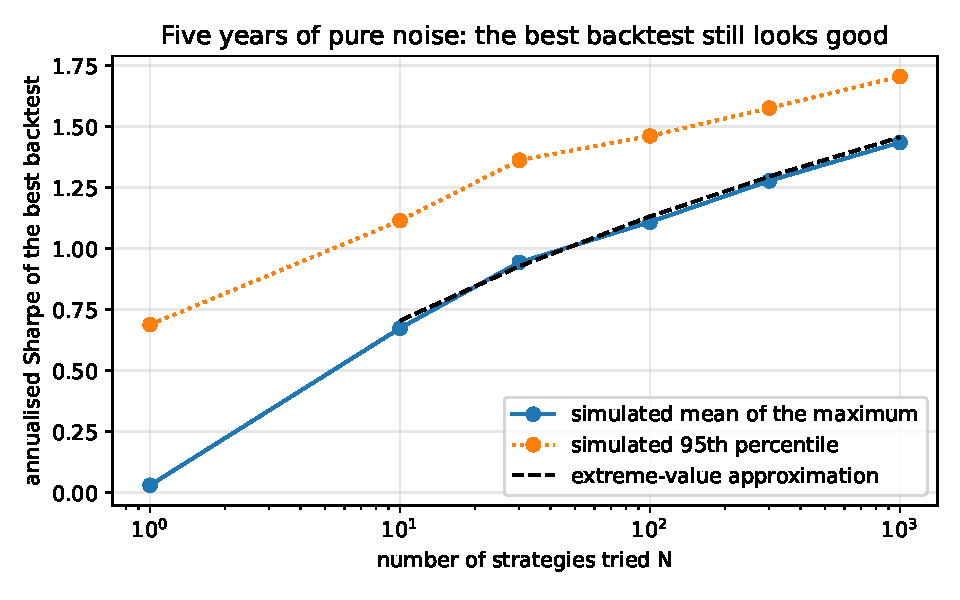
\includegraphics[width=0.78\textwidth]{figures/max_sharpe.pdf}
\caption{Annualised Sharpe ratio of the best backtest among $N$ strategies with zero true Sharpe.}\label{fig:max}
\end{figure}

\begin{table}[H]\centering\small
\begin{tabular}{lrrrrrr}
\toprule
$N$ & 1 & 10 & 30 & 100 & 300 & 1000\\
\midrule
Simulated mean of the maximum & 0.03 & 0.67 & 0.94 & 1.11 & 1.28 & 1.44\\
Approximation \eqref{eq:emax} & 0 & 0.70 & 0.93 & 1.13 & 1.30 & 1.46\\
Simulated 95th percentile & 0.69 & 1.11 & 1.36 & 1.46 & 1.58 & 1.71\\
\bottomrule
\end{tabular}
\caption{Maximum annualised Sharpe ratio of null strategies, five years of daily data.}
\end{table}

The approximation is within 5\% of the simulated mean from $N=10$ upwards. The growth is slow, roughly as $\sqrt{2\ln N}$, which is why the problem is easy to underestimate: going from 100 to 1\,000 trials adds only 0.3 to the expected maximum, but by then the expected maximum already exceeds what most real strategies deliver. A researcher who reports a Sharpe of 1.4 after trying a thousand variants has shown nothing.

\section{Testing the selected strategy}
In each of 400 simulations, 100 null strategies are generated, the best is selected, and two tests are applied: PSR against zero and the deflated Sharpe ratio, both with a 95\% threshold.

The naive PSR rejects the null in 99.5\% of simulations, against a nominal 5\%. The deflated Sharpe ratio rejects it in 0.5\% of simulations. It is therefore conservative rather than exact: the benchmark is the expected maximum, and a 95\% threshold on top of that asks the selected strategy to beat the typical luck by a further margin.

Figure~\ref{fig:power} then plants one real strategy among the 100 and varies its true Sharpe ratio.

\begin{figure}[H]\centering
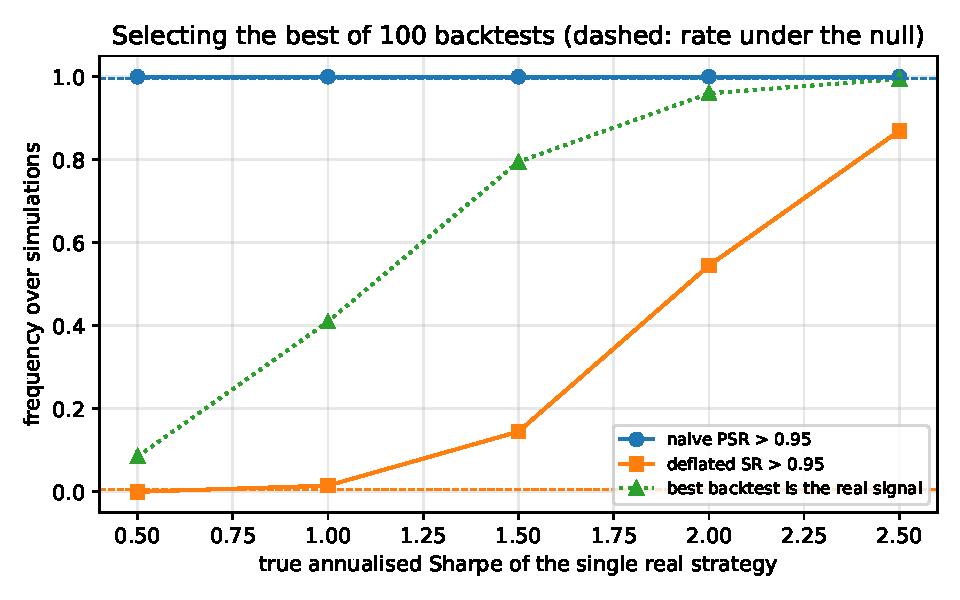
\includegraphics[width=0.78\textwidth]{figures/dsr_power.pdf}
\caption{Rejection rates when one of 100 strategies is real (200 simulations per point).}\label{fig:power}
\end{figure}

\begin{table}[H]\centering\small
\begin{tabular}{lrrrrr}
\toprule
True annualised Sharpe of the real strategy & 0.5 & 1.0 & 1.5 & 2.0 & 2.5\\
\midrule
Best backtest is the real strategy & 8.5\% & 41\% & 80\% & 96\% & 99.5\%\\
Deflated SR $>0.95$ & 0\% & 1.5\% & 14.5\% & 54.5\% & 87\%\\
Naive PSR $>0.95$ & 100\% & 100\% & 100\% & 100\% & 100\%\\
\bottomrule
\end{tabular}
\caption{Selection and detection of a single real strategy among 100.}
\end{table}

Two observations follow. First, the naive test has no discriminating power: it rejects whether or not a real strategy exists. Second, the difficulty is not in the test but in the data. With a true Sharpe of 1.0, the best backtest is the real strategy in only 41\% of simulations; in the remaining 59\% a noise strategy beat it, and no test applied afterwards can recover that. Five years of daily data are not enough to identify a Sharpe-1 strategy among a hundred candidates. The remedies are more data, fewer trials, or an economic prior that reduces the number of candidates before testing.

\section{Controlling a universe of signals}
The next experiment tests 1\,000 strategies, 50 of which have a true Sharpe ratio of 1.0, using a one-sided $z$-test for each. Table~\ref{tab:mt} averages 200 simulations.

\begin{table}[H]\centering\small
\begin{tabular}{lrrr}
\toprule
Procedure & FDR & Power & FWER\\
\midrule
No correction ($p<0.05$) & 56.5\% & 72.7\% & 100\%\\
Bonferroni & 2.6\% & 4.9\% & 6.5\%\\
Holm & 2.6\% & 4.9\% & 6.5\%\\
Benjamini--Hochberg & 5.6\% & 13.1\% & 33\%\\
\bottomrule
\end{tabular}
\caption{1\,000 strategies, 50 real with Sharpe 1.0, five years of data, $\alpha=5\%$.}\label{tab:mt}
\end{table}

Without correction the procedure finds most of the real strategies, but more than half of what it reports is noise, and a false discovery occurs in every simulation. Bonferroni and Holm behave identically here, because Holm only departs from Bonferroni after the first rejections, and there are very few. Benjamini--Hochberg nearly triples the power for an FDR that stays close to its target.

Two figures are slightly above their theoretical bounds. With 950 null strategies, Bonferroni guarantees a FWER of at most $4.75\%$ and Benjamini--Hochberg an FDR of at most $4.75\%$; the simulations give 6.5\% and 5.6\%. Part of the gap is sampling error: with 200 simulations the standard error of a 5\% frequency is about 1.5 points. Part may come from the $p$-values themselves, which rely on the normal approximation of the Sharpe estimator and are evaluated far in the tail, near $5\times10^{-5}$ for Bonferroni, where the approximation is least reliable. Separating the two effects would require more simulations or exact $t$-test $p$-values; this has not been done.

\section{Probability of backtest overfitting}
The CSCV procedure is applied to four years of daily data, 100 strategies and $S=12$ blocks, giving 924 splits per dataset. Figure~\ref{fig:pbo} shows one dataset for each configuration.

\begin{figure}[H]\centering
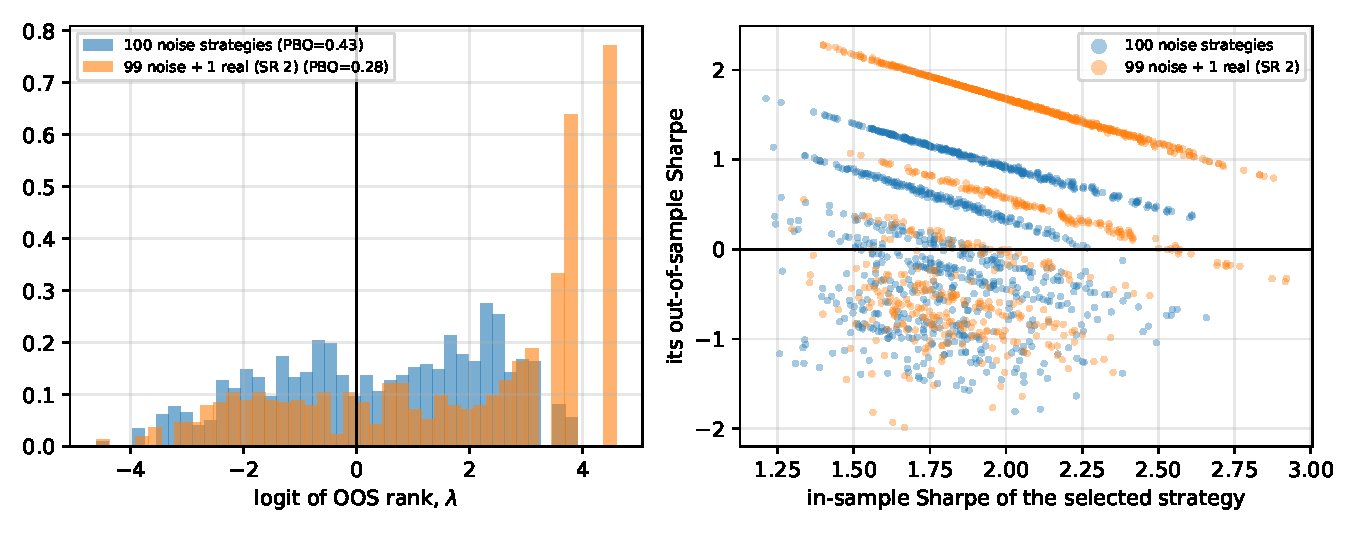
\includegraphics[width=\textwidth]{figures/pbo.pdf}
\caption{Left: distribution of the logits $\lambda$ over the 924 splits. Right: in-sample against out-of-sample Sharpe of the selected strategy.}\label{fig:pbo}
\end{figure}

For the noise universe, the selected strategy has a median in-sample Sharpe of 1.82 and a median out-of-sample Sharpe of 0.28, and PBO is 0.43. When one strategy has a true Sharpe of 2, the median out-of-sample Sharpe of the selected strategy rises to 1.22 and PBO falls to 0.28. The right panel shows the mechanism: in the noise case the out-of-sample performance of the selected strategy is unrelated to its in-sample performance, while in the second case a cluster of splits selects the real strategy and keeps its performance.

A single PBO value is however a statistic computed from one dataset. Repeating the procedure on 20 independent datasets gives:

\begin{table}[H]\centering\small
\begin{tabular}{lrrrr}
\toprule
Universe & Mean PBO & Std & Min & Max\\
\midrule
100 noise strategies & 0.47 & 0.15 & 0.23 & 0.70\\
99 noise + 1 real (Sharpe 2) & 0.23 & 0.19 & 0.01 & 0.62\\
\bottomrule
\end{tabular}
\caption{Variability of PBO across 20 independent datasets.}
\end{table}

On average the method separates the two cases, but the ranges overlap widely: some noise datasets give a PBO of 0.23 and some datasets containing a real strategy give 0.62. The splits within one dataset are strongly dependent, since they reuse the same returns, so the 924 logits carry much less information than their number suggests. PBO is best used to compare research processes on the same data, not as an absolute pass/fail threshold.

\section{Fat tails and the standard error}
Equation~\eqref{eq:var} corrects the standard error for skewness and kurtosis. To see whether this matters for daily data, 4\,000 one-year samples with a true Sharpe of 1.0 were drawn from normal and from Student-$t$ distributions with 3.5 degrees of freedom, and the coverage of 95\% confidence intervals was measured.

\begin{table}[H]\centering\small
\begin{tabular}{lrr}
\toprule
Return distribution & Normal formula & Moment-adjusted formula\\
\midrule
Normal & 95.3\% & 95.2\%\\
Student-$t$, 3.5 d.o.f. & 94.4\% & 93.2\%\\
\bottomrule
\end{tabular}
\caption{Coverage of 95\% confidence intervals for the daily Sharpe ratio.}
\end{table}

The correction does not help here, and in the fat-tailed case it makes the coverage slightly worse. The reason is visible in equation~\eqref{eq:var}: the daily Sharpe ratio is about $0.06$, so the kurtosis enters through a term of order $SR^2\approx0.004$ and has almost no effect, while the sample kurtosis of a Student-$t$ with 3.5 degrees of freedom is very unstable because the fourth moment of that distribution is infinite. The adjustment matters for skewed returns and for lower frequencies, where the per-period Sharpe ratio is larger; for symmetric daily returns the simple formula is adequate.

%--------------------------------------------------------------------------
\chapter{Limits and Extensions}

The strategies simulated here are independent. Real strategies built from the same data are correlated, which reduces the effective number of trials: the expected maximum of 1\,000 correlated backtests is lower than that of 1\,000 independent ones, and Bonferroni becomes more conservative still. Estimating an effective number of independent trials, for instance by clustering the strategy returns, is the natural next step.

Returns are also i.i.d.\ in time. Autocorrelation changes the standard error of the Sharpe ratio, and contiguous blocks in CSCV only partly protect against it. Finally, the selection rule is always the maximum in-sample Sharpe; real research processes are less mechanical, which is precisely why a method such as PBO, which does not need to count the trials, is attractive despite its variance.

The same tools will be applied to the cross-sectional equity signals of the alpha research project in progress, where the number of variants tested is the main source of risk.

\chapter*{References}
\addcontentsline{toc}{chapter}{References}
\begin{enumerate}[label={[\arabic*]},leftmargin=2em]
\item A. W. Lo, \emph{The Statistics of Sharpe Ratios}, Financial Analysts Journal 58(4) (2002).
\item E. Mertens, \emph{Comments on Variance of the IID Estimator in Lo (2002)}, working paper (2002).
\item D. H. Bailey and M. López de Prado, \emph{The Sharpe Ratio Efficient Frontier}, Journal of Risk 15(2) (2012).
\item D. H. Bailey and M. López de Prado, \emph{The Deflated Sharpe Ratio: Correcting for Selection Bias, Backtest Overfitting and Non-Normality}, Journal of Portfolio Management 40(5) (2014).
\item D. H. Bailey, J. M. Borwein, M. López de Prado and Q. J. Zhu, \emph{The Probability of Backtest Overfitting}, Journal of Computational Finance 20(4) (2017).
\item Y. Benjamini and Y. Hochberg, \emph{Controlling the False Discovery Rate}, J. Royal Statistical Society B 57(1) (1995).
\item C. R. Harvey, Y. Liu and H. Zhu, \emph{\ldots and the Cross-Section of Expected Returns}, Review of Financial Studies 29(1) (2016).
\end{enumerate}

\chapter*{Appendix: Key Functions}
\addcontentsline{toc}{chapter}{Appendix: Key Functions}
The full code, the tests and the experiment script are in the repository.

\section*{Expected maximum and deflated Sharpe ratio}
\lstinputlisting[linerange={39-54},firstnumber=39]{../src/bto/sharpe.py}

\section*{CSCV estimate of PBO}
\lstinputlisting[linerange={25-44},firstnumber=25]{../src/bto/pbo.py}

\end{document}
